\documentclass[border=6pt]{standalone}
\usepackage{amsmath}
\usepackage{amssymb}
\usepackage{tikz}
\usepackage{xcolor}
\usetikzlibrary{arrows.meta,calc,positioning,shapes.geometric}
\begin{document}
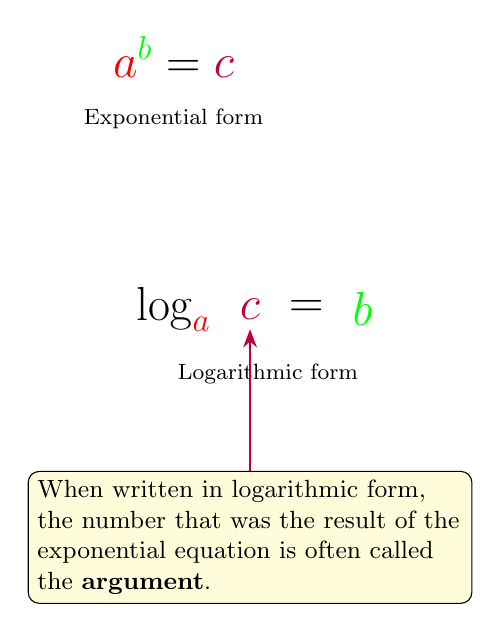
\begin{tikzpicture}[font=\sffamily]
  % Exponential form
  \node[font=\LARGE] (expform) at (0,3.2) {$\textcolor{red}{a}^{\textcolor{green}{b}} = \textcolor{purple}{c}$};
  \node[below=0.15cm of expform, font=\footnotesize] {Exponential form};

  % Logarithmic form, built piece-by-piece so an arrow can target c precisely
  \node[font=\LARGE] (logpart1) at (0,0) {$\log_{\textcolor{red}{a}}$};
  \node[font=\LARGE, right=0.12cm of logpart1] (logc) {$\textcolor{purple}{c}$};
  \node[font=\LARGE, right=0.12cm of logc] (logeq) {$=$};
  \node[font=\LARGE, right=0.12cm of logeq] (logb) {$\textcolor{green}{b}$};
  \node[font=\footnotesize] at ($(logpart1.south)!0.5!(logb.south)+(0,-0.45)$) {Logarithmic form};

  % callout pointing at c
  \node[draw, rounded corners=4pt, fill=yellow!15, text width=5.4cm, align=left,
        font=\small, below=1.8cm of logc] (callout)
        {When written in logarithmic form, the number that was the result of the
         exponential equation is often called the \textbf{argument}.};
  \draw[-Stealth, thick, purple] (callout.north) to[out=90,in=270] (logc.south);
\end{tikzpicture}
\end{document}
